\documentclass[12pt]{cours}

\title{\textbf{\textsc{Diagramme des classes}}}
\author{Delay Emmanuel -- Desforêts Nicolas}


\usepackage{pgf-umlcd}



\begin{document}

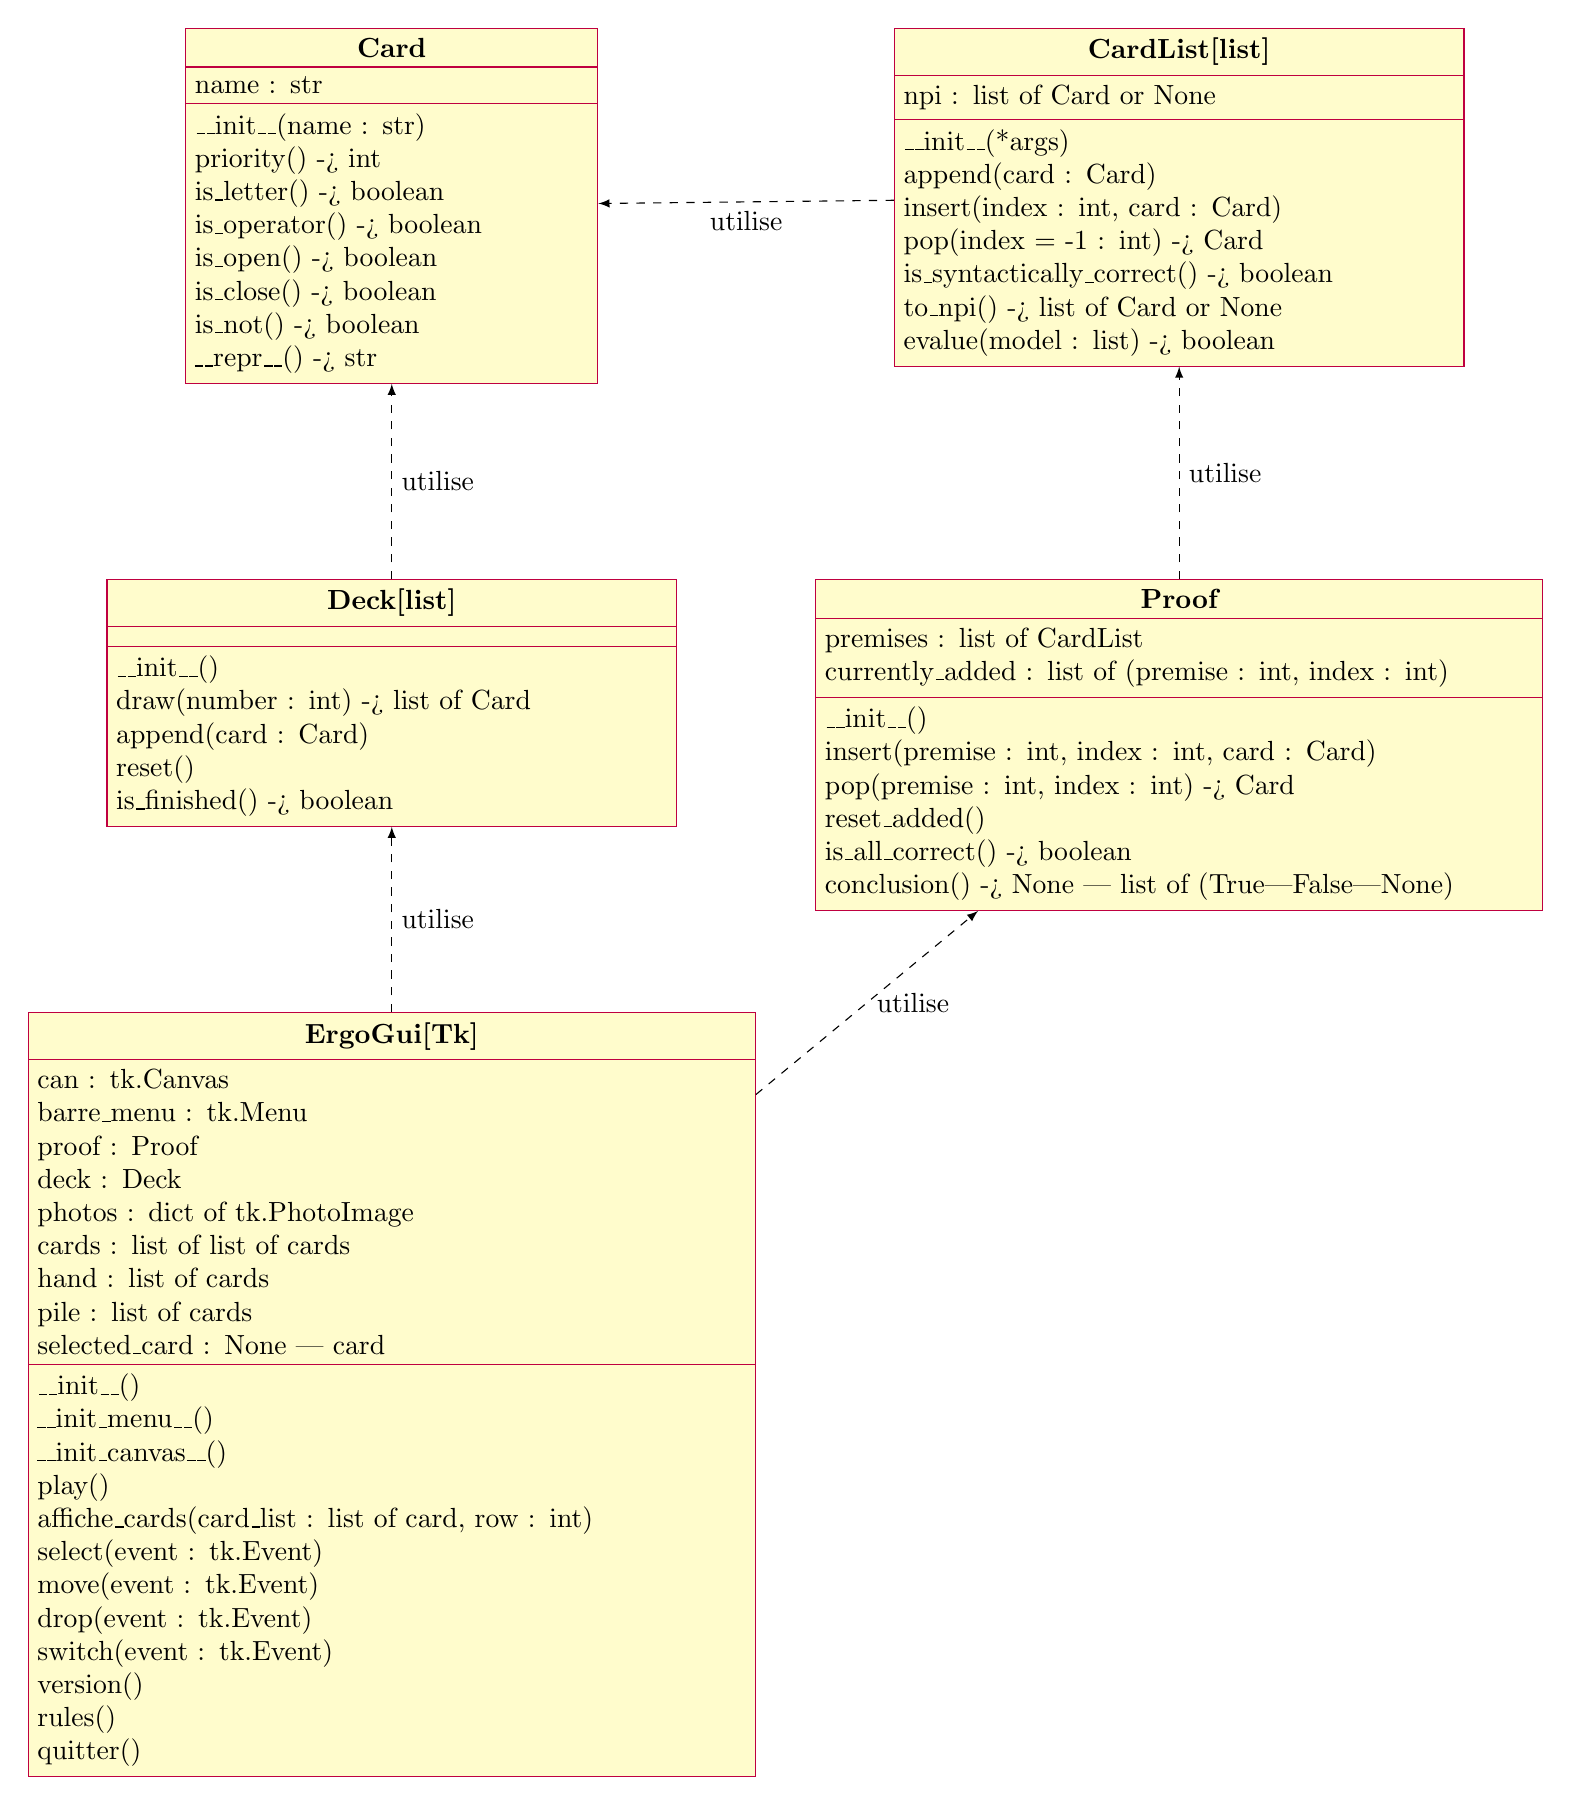
\begin{tikzpicture}
\begin{class}{Card}{0, 0}
\attribute{name : str}
\operation{\_\_init\_\_(name : str)}
\operation{priority() -> int}
\operation{is\_letter() -> boolean}
\operation{is\_operator() -> boolean}
\operation{is\_open() -> boolean}
\operation{is\_close() -> boolean}
\operation{is\_not() -> boolean}
\operation{\_\_repr\_\_() -> str}
\end{class}

\begin{class}[text width=7cm]{CardList[list]}{10,0}
\attribute{npi : list of Card or None}
\operation{\_\_init\_\_(*args)}
\operation{append(card : Card)}
\operation{insert(index : int, card : Card)}
\operation{pop(index = -1 : int) -> Card}
\operation{is\_syntactically\_correct() -> boolean}
\operation{to\_npi() -> list of Card or None}
\operation{evalue(model : list) -> boolean}
\end{class}

\draw[dashed,-latex] ({CardList[list]}) -- node[below, midway]{utilise} (Card);

\begin{class}[text width=9cm]{Proof}{10, -7}
\attribute{premises : list of CardList}
\attribute{currently\_added : list of (premise : int, index : int)}
\operation{\_\_init\_\_()}
\operation{insert(premise : int, index : int, card : Card)}
\operation{pop(premise : int, index : int) -> Card}
\operation{reset\_added()}
\operation{is\_all\_correct() -> boolean}
\operation{conclusion() -> None | list of (True|False|None)}
\end{class}

\draw[dashed,-latex] (Proof) --node[right, midway]{utilise} ({CardList[list]});

\begin{class}[text width=7cm]{Deck[list]}{0,-7}
\operation{\_\_init\_\_()}
\operation{draw(number : int) -> list of Card}
\operation{append(card : Card)}
\operation{reset()}
\operation{is\_finished() -> boolean}
\end{class}

\draw[dashed,-latex] ({Deck[list]}) --node[right, midway]{utilise} (Card);

\begin{class}[text width=9cm]{ErgoGui[Tk]}{0,-12.5}
\attribute{can : tk.Canvas}
\attribute{barre\_menu : tk.Menu}
\attribute{proof : Proof}
\attribute{deck : Deck}
\attribute{photos : dict of tk.PhotoImage}
\attribute{cards : list of list of cards}
\attribute{hand : list of cards}
\attribute{pile : list of cards}
\attribute{selected\_card : None | card}
\operation{\_\_init\_\_()}
\operation{\_\_init\_menu\_\_()}
\operation{\_\_init\_canvas\_\_()}
\operation{play()}
\operation{affiche\_cards(card\_list : list of card, row : int)}
\operation{select(event : tk.Event)}
\operation{move(event : tk.Event)}
\operation{drop(event : tk.Event)}
\operation{switch(event : tk.Event)}
\operation{version()}
\operation{rules()}
\operation{quitter()}
\end{class}

\draw[dashed,-latex] (ErgoGui[Tk]) --node[right, midway]{utilise} ({Deck[list]});
\draw[dashed,-latex] (ErgoGui[Tk]) --node[right, midway]{utilise} (Proof);
\end{tikzpicture}


\end{document}

